%\documentclass[aps,prl,preprint,superscriptaddress,showpacs]{revtex4}
\documentclass[aps,prl,reprint,longbibliography,superscriptaddress, english]{revtex4-1}
%\documentclass[aps,prl,reprint,longbibliography]{revtex4-1}
%\usepackage{graphicx}
 \usepackage[utf8]{inputenc}
 \usepackage{amsmath,bm}
 \usepackage{mathrsfs}
 \usepackage{amsfonts}
 %\usepackage[font=it]{caption}
 \usepackage{graphicx}
 %\usepackage{xcolor}
 \usepackage{setspace} %leaves captions single space in draft mode
 \usepackage{graphicx}
 \usepackage{epstopdf}
 \usepackage{dcolumn}
 \usepackage{amsmath}
 \usepackage{epsfig}
 \usepackage{indentfirst}
 \usepackage{psfrag}
 \usepackage{subfigure}
 %\usepackage{subcaption}
 \usepackage{amssymb}
 %\bibliographystyle{apsrev}
 \usepackage{color}
 \usepackage{units} % rz
\usepackage{soul} % strikethrough text
\usepackage{siunitx}
 \usepackage{graphicx}% Include figure files
 \usepackage{float}
 \graphicspath{{Figures/}} %Setting the graphicspath
 \usepackage{dcolumn}% Align table columns on decimal point
 \usepackage{bm}% bold math
 \usepackage{multirow}

\usepackage{physics}
\usepackage{dcolumn}% Align table columns on decimal point
\usepackage{bm}% bold mathhttps://www.overleaf.com/project/5af95d0f3775594d14d4a052
%\usepackage{hyperref}% add hypertext capabilities
\usepackage{natbib}
\usepackage[backref=none,bookmarksnumbered=true,bookmarks=true,bookmarksopen=true,colorlinks=true,
citecolor=blue,linkcolor=blue,anchorcolor=green,urlcolor=blue,unicode=false]{hyperref}

%******************************* For corrections ===================
\usepackage{ulem}[normalem] %Whatch out, places underlining in Journal references. Use \normalem before references to deactivate this 
\def\red{\color{red}}
\def\black{\color{black}}
\def\blue{\color{blue}}
\def\BappCl{BaCl$_2$ }
%\def\Bapp{Ba$^{+2}$ }
%\def\Nap{Na$^{+}$ }


\normalem
\newcommand{\np}[1]{\textcolor{blue}{ #1}}
\newcommand{\npc}[1]{\textcolor{cyan}{(NP: #1)}}
\newcommand{\rw}[1]{\textcolor{cyan}{RW: #1}}
\newcommand{\str}[1]{\textcolor{cyan}{\st{#1}}}

\newcommand{\completar}[1]{{\color{red} #1}}
\newcommand{\rev}[1]{{\color{blue} #1}}

\makeatletter
\newcommand\colorsout[1]{\bgroup \markoverwith{\textcolor{#1}{\rule[0.5ex]{2pt}{0.4pt}}}\ULon}
\newcommand{\effacer}[1]{{\colorsout{red}{{\color{red}#1}}}}
\makeatother
%******************************* For corrections ===================


%******************************* Supporting Info ===================
\newcommand{\beginsupplement}{%
        \setcounter{table}{0}
        \renewcommand{\thetable}{S\arabic{table}}%
        \setcounter{figure}{0}
        \renewcommand{\thefigure}{S\arabic{figure}}%
     }
%******************************* Supporting Info ===================


\input{NextDefs.tex}

\begin{document}
\title{Demonstration of the detection of \Bapp\ ions with molecular sensors for an ultra-low background neutrinoless double beta decay experiment}

   \author{Pablo Herrero}
   \affiliation{Centro de F\'{\i}sica de Materiales (CSIC/UPV-EHU), 20018 Donostia-San Sebasti\'an, Spain}
   \affiliation{Donostia International Physics Center DIPC, 20018 Donostia-San Sebasti\'an, Spain}
   \author{Maxim Ilyn}
   \affiliation{Centro de F\'{\i}sica de Materiales (CSIC/UPV-EHU), 20018 Donostia-San Sebasti\'an, Spain}
    \author{Martina Corso}
   \affiliation{Centro de F\'{\i}sica de Materiales (CSIC/UPV-EHU), 20018 Donostia-San Sebasti\'an, Spain}
   \affiliation{Donostia International Physics Center DIPC, 20018 Donostia-San Sebasti\'an, Spain}

    \author{Dimas's group people}
   \affiliation{Centro de F\'{\i}sica de Materiales (CSIC/UPV-EHU), 20018 Donostia-San Sebasti\'an, Spain}
   \affiliation{Donostia International Physics Center DIPC, 20018 Donostia-San Sebasti\'an, Spain}
 \author{Sospechosos habituales}
   \affiliation{Donostia International Physics Center DIPC, 20018 Donostia-San Sebasti\'an, Spain}
\affiliation{UPV-EHU}

  \author{Celia Rogero}
   \affiliation{Centro de F\'{\i}sica de Materiales (CSIC/UPV-EHU), 20018 Donostia-San Sebasti\'an, Spain}
   \affiliation{Donostia International Physics Center DIPC, 20018 Donostia-San Sebasti\'an, Spain}


\begin{abstract}

Neutrinos are the only elementary particles that could be their own antiparticles\cite{Majorana:1937}. This could be stablished experimentally by observing neutrinoless double beta decays in a number of isotopes\cite{GomezCadenas:2010gs}. Experiments attempting to see this rare reaction must suppress by many orders of magnitude the huge background associated to natural radioactivity. Xenon-based Time Projection Chambers could achieve this feat by identifying --``tagging"-- the  daughter \Bapp\ ion produced in the decay\cite{Moe:1991ik,Nygren_2015, Jones:2016qiq, McDonald:2017izm, Chambers:2018srx}. In particular, the use of a fluorescent bicolor indicator (FBI) has been recently proposed as the building block of barium tagging sensor\cite{rivilla_fluorescent_2020}. Here we use a combination of surface science techniques to measure the formation of supramolecular complexes  in monolayers of FBI sensors under vacuum conditions, thus unambiguously demonstrating the feasibility of the FBI indicator to capture and identify \Bapp\ ions. 
%The molecules, immobilized on a surface, can trap different ions, \Bapp or \Nap ions, and  this process alters the molecular core level peaks, the structural conformation, as well as the electronic molecular structure, as revealed by the combination of XPS and STM/STS.
\end{abstract}

\date{\today}
\maketitle

\section*{}

The rare decay called neutrinoless double beta  (\bbonu) decay, $(Z,A) \rightarrow (Z+2,A) + 2\ e^{-}$ can occur if and only if neutrinos are Majorana particles \cite{Majorana:1937}, e.g., identical to their antiparticles. An unambiguous observation of such decay would have deep implications in particle physics and cosmology\cite{Sakharov1967,Fukugita:1986hr, GellMann:1980vs, Yanagida:1979as, Mohapatra:1979ia}. 

A rich experimental program has been conducted over more than fifty years, searching, so far unsuccessfully, for such decays, in a variety of isotopes. In particular, experiments based in the \XE\ isotope have yielded an upper limit on the \bbonu\ lifetime $\Tonu > 10^{26}$ \si{\year} \cite{Gando:2016ji}.  An intense effort is underway to improve the sensitivity to \Tonu\ by at least one, and eventually two orders of magnitude \cite{Gomez-Cadenas:2019sfa}. These searches will require very large exposures, measured in ton-years, but even more importantly, 
a greatly enhanced capability to suppress  spurious events. 

The most obvious background to \bbonu\ is the \bbtnu\ decay, $(Z,A) \rightarrow (Z+2,A) + 2\ e^{-} + 2\ \nu$, which also produces two electrons and the same daughter atom as in the neutrinoless mode, while having a much faster decay rate. Near the end point energy  (\Qbb), however, the \bbtnu\ process is very strongly suppressed by kinematics and its contamination to the \bbonu\ signal turns out to be very small for a detector with good energy resolution \cite{Elliott:2002xe}.  
Instead, due to the irreducible presence of trace amounts of the radioactive decays chains of \URANIUM\ and \THO\ in materials of the detector, their false signatures need to be suppressed by many orders of magnitude.  

The most powerful discriminant against backgrounds other than \bbtnu\ would be the detection of the daughter atom. In particular, the decay $\XE \rightarrow Ba  + 2\ e \, (+ 2\ \overline{\nu}_{e})$, will create a \Bapp\ dication as the most likely outcome in xenon gas. In pure xenon gas, no known radioactive process will produce the appearance of this ion, {\it in  coincidence with two electrons}. 

In a recent publication, the use of a new fluorescent bicolor indicator (FBI) 
was proposed as the core of a sensor able to detect single \Bapp\ ions in a
high-pressure gas detector\cite{rivilla_fluorescent_2020}. The indicator is synthesised to bind strongly to \Bapp\ 
and to shine very brightly when complexed with \Bapp. Furthermore, the emission spectrum of the chelated indicator is significantly blue-shifted  with respect to the unchelated species, allowing an additional discrimination of almost two  orders of magnitude. 

Chemical sensors are miniaturised devices that can deliver real time and on-line information on the presence of specific compounds or ions in even complex samples \cite{cammann1996cambridge}. 
Among them, optical chemical sensors employ optical transduction techniques to yield analyte information \cite{mcdonagh_optical_2008}. Due to the outstanding characteristics of both fluorescence and phosphorescence signals, they are widely applied to the construction of  sensors where susceptible fluorescence molecules are immobilised on a surface \cite{wolfbeis_materials_2005}.This kind of sensors has been used in many different applications in biology, medicine, environment,  \completar{.... Completar aplicaciones y referencias}. 
 
In the last few years, fluorescence chemo-sensors have been proposed as the cornerstone of a detector able to identify single \Bapp\ ions in a high pressure xenon TPC\cite{Nygren_2015, Jones:2016qiq, McDonald:2017izm, thapa_barium_2019, thapa_demonstration_2021}. A crucial feature of such sensors (also known as indicators), is their capability to signal the presence of the complexed system (often referred to as the chelated molecule) from the ree (unchelated) state. Recently, the use of a new fluorescent bicolor indicator (FBI) 
has been proposed as an excellent candidate for a \Bapp\ detector \cite{rivilla_fluorescent_2020}. This molecule (shown schematically in the upper panel of figure \ref{ModeloFBI}), has a crown ether derivative group ---which actas as trapping cage for the ions--- bonded to a custom-designed fluorophore. The molecule offers a strong selectivity for capturing \Bapp\ and a very characteristic signal upon chelation. When a \Bapp\ ion is captured, not only the crown ether but also the phenyl group and the nitrogen contained in the fluorophore participate in the coordination bond with the  ion. This coordination induces a large molecular torsion with respect to the free  molecule. As a result, the fluorescence emission spectrum gets considerably blue-shifted. This blue-shift has been precisely measured in solution, and provides a very robust separation between chelated and free states.

Notice that there are important difference between the chemo-sensors needed for a \bbonu\ experiment based in a high pressure xenon TPC and those used routinely in biochemistry. In the late case, the chelation and detection process occurs in aqueous solution, while in the \bbonu\ experiment one needs to prepare a suitable surface, functionalise it with sensors, and operate it in dry medium (noble gas). It is, therefore, imperative to show that chelation of the candidate indicators occurs in thin molecular layers in the absence of any solvent ---in that respect, good vacuum qualifies as the perfect dry medium---. A first proof of concept was presented in \cite{rivilla_fluorescent_2020}: FBI molecules were deposited over a silica pellet, and barium perchlorate was sublimated over that surface, using a Knudsen cell. Examination of the test pellet before and after sublimation showed a strong blue shift, indicating that a large fraction of the molecules were chelated. However, the experiment had several limitations. First, the distribution of FBI molecules over the silica substrate was very irregular, and the density of indicators in such surface was not well known. Second, the examination of the sample after chelation was done outside the Knudsen chamber. This could raise doubts concerning whether the iteration of the indicators, and the Ba(ClO$_4$)$_2$ could be affected by exogenous agents, such as, for example, ambient water vapor. Furthermore, while in the response of FBI to metals other than \Bapp\ was studied, showing high specificity for the later, those studies were carried out in solution. 


%, we take further steps towards the development of a \Bapp\ detector based in FBI chemo-sensors. As discussed above, such a detector will require the immobilisation of thin molecular layers on a suitable surface, while preserving its capability for ion capture. The process must take place in the absence of any solvent since the sensor will be installed in a high-pressure gas xenon chamber. If vacuum is used as dry medium, is also desirable that demonstration of chelation is performed without breaking it. Last but not least, it is important to characterise the conformational changes that occur in the molecule upon chelation and compare them with theoretical calculations. By combining 
 
 \begin{figure*}[ht!]
	\includegraphics[width=0.9\textwidth]{figures/fig1_fbi_model.pdf}
	\caption{\label{ModeloFBI} 
    Upper panel: Model of the FBI molecules before and after chelation, including the fluorescence colours in solution. Lower panel: schematic representation of the experiment we have carried out, where FBI molecules were sublimated, chelated and characterised inside the UHV chamber.}
\end{figure*}  

In this paper we combine highly sensitive surface techniques, including X-ray Photoemission Spectroscopy (XPS) and Scanning Tunnelling Microscopy and Spectroscopy (STM/STS), to prove how different ions interact with FBI molecules deposited in thin layers upon suitable substrates. We demonstrate that only \Bapp\ ions induce molecular structural changes, modifying the electronic structure and therefore affect the fluorescence emission. Coordination with crown-ether happens entirely in vacuum, which ensures that chemical, structural and electronic changes are independent of solvents, air molecules or spurious contaminants. This is, therefore, a crucial step toward the development of a \Bapp\ detector. 
%Furthermore, it provides the bases to envision the application of this kind of crown ether-based chemosensors in a broad development of sensing, such as the detection of Ra atoms.

In addition, the work presented here, advances substantially the understanding of Crown ethers immobilised in solid surfaces. 
This macrocyclic molecules are very important in applications such as drug carriers \cite{uchegbu_non-ionic_1998} or photo-switching devices \cite{malval_photoswitching_2002}, \cite{uda_membrane_2005}. Because of their capability to capture a variety of guest species, including metal cations, protonated species and neutral and ionic molecules \cite{dobler1980ionophores}, crown ethers \cite{gokel_crown_1991} have been extensively used in solution, or even in gas phase to recognise and trap metal or molecular ions \cite{more_intrinsic_1999}, \cite{maleknia_cavity-size-dependent_2002}. However, despite their unique coordinating properties, crown ethers have been poorly exploited in solid state. Few examples can be found in the literature where self-assembled monolayers of crown ether derivatives have been grown and used on surfaces. Moreover, in all previous studies, either the growth or ion trapping or both has taken place in solution \cite{yoshimoto_hostguest_2003}, \cite{flink_recognition_1999}, \cite{inokuchi_new_2015}. 
 There are only two works, as far as we know, where crown ethers were deposited under ultra high vacuum conditions (UHV) \cite{feng_growth_2018} and their metal trapping capability was proven also under UHV \cite{stredansky_-surface_2019}. In the latter work, reactivity of the crowns upon anchoring on an organic template on Au(111) is carefully explored. In addition, by combining XPS and STM, they probe that the crown ethers, assembled into a regular 2D guest--host array, can successfully trap sodium atoms.

%\section{Results and discussion}
%Esta separación por apartados/subapartados luego puede aparecer o no, dependiendo de a que revista lo mandemos, pero por ahora la dejo porque ayuda a escribir y ordenar las ideas. Luego se puede reestructurar para que el mensaje llegue de la mejor manera posible.

\section{Sublimation of molecules}
For our initial studies, FBI molecules were sublimated on a gold substrate (see lower panel of figure \ref{ModeloFBI}). The first step was 
to confirm that the sublimated molecules were intact on the substrate. Figure \ref{XPS_FBI_Au(111)} a) shows the molecular core levels of FBI, i.e. $O 1s$, N 1s and C 1s. The spectra were measured for 0.65 ML deposited on Au(111) at RT. The ratios between the three core levels are in agreement with having stoichiometric molecules on the surface (C/O = 6.2, C/N = 10.3). The C 1s core level, which appears centred at around 285 eV, can be fitted using two components, one centred at around 284.7 eV and a second and more intense one at 286.3 eV, with relative intensities in agreement with having intact molecules. The former component corresponds to C-C bonds whereas the component at higher binding energy (B.E.) includes contributions from C-O and C-N. In the N 1s region, around 400 eV, a faint peak is visible. The position of the maxima is compatible with the two amida groups of the molecular composition. Finally, the O 1s core level present a single component peak centred at 532.8 eV.

\begin{figure*}[ht!]
	\includegraphics[width=0.9\textwidth]{figures/fig2_xps_chelation.a).png}
	\includegraphics[width=0.4\textwidth]{figures/XPS_O1s_evolution_Au.png}
	
	%\includegraphics[width=0.5\textwidth]{XPS_O1s_evolution_Au.png}
	\caption{\label{XPS_FBI_Au(111)} 
    XPS spectra on O 1s, N 1s and C 1s regions measured after 0.65 ML FBI deposition on Au(111) (a); after their chelation with 1.46 \Bapp per FBI molecule (b) and 1.43 \Nap per FBI molecule (c). Evolution of chelated component as a function of the \Bapp deposition (d)}
\end{figure*}  

\section{Chemical probe of chelation}
For the chelation, \BappCl was sublimated on the FBI-functionalised Au(111) surface. It is worth mentioning that upon sublimation, the stoichiometry of the salt does not remain 1:2 but rather 2:1. This means that mainly \Bapp\ is deposited on the surface (see S.I. for details).
After sublimation of 1.46 \Bapp per FBI molecule, the core levels, shown in figure \ref{XPS_FBI_Au(111)} b), are clearly shifted toward higher B.E, mainly on O 1s and N 1s

The maximum O 1s core level exhibits an upward shift of 0.5 eV. This shift is not just a doping shift, but a real chemical change. This is revealed by the evolution of the O 1s for very low \Bapp doses on the surface. Figure \ref{XPS_FBI_Au(111)} shows the O 1s evolution for \Bapp ions amounts below 1 \Bapp per FBI molecule. The peak width increases as \Bapp is added to the sample: the peak of the free molecule (prior to \Bapp addition) has a FWHM of 2.04, whereas it has a FWHM of 2.20 for the lattest state, with 0.63 \Bapp per FBI. Thus, we deconvolve the peaks after \Bapp addition using two components, one at 533.2 eV (FWHM = 2.20) corresponding to the free molecules and another at 533.8-534.0 eV, corresponding to chelated molecules.   This is consistent with the molecules undergoing a chemical change upon chelation, rather than a surface doping shift due to adding the ions. \completar{The relative contribution of the component from the chelated molecules may be expected to depend on the amount of barium deposited. However, the resolution of the current experiments limited our assessment of this dependency.}. The contribution to the O 1s peak from the neighbouring Au 4p was subtracted using the spectrum of the clean Au. More information can be found in the supplementary information.

In the only reference paper were crown ether deposited on Au(111) were chelated, ref. \cite{stredansky_-surface_2019} Stredansky and coworkers observed higher shifts in the O1s core level, which gradually shifts up to around 1 eV by increasing the amount of deposited atoms (\Nap in their case). 
To evaluate whether the nature of the dopant atom has any influence in the oxygen core level shift for the FBI molecules, we tested the chelation with Na. Thus, figure \ref{XPS_FBI_Au(111)} c) shows the O 1s, N 1s and C 1s core levels measured on 0.6 ML of FBI on Au(111) before and after the sublimation of 1.43 \Nap per FBI. The maximum O 1s shift for \Nap-chelated FBI molecules is again 0.5 eV, excluding the nature of the ion as responsible of the shift.
It is noteworthy to remember here that in REF \cite{stredansky_-surface_2019} crown ether groups were oriented parallel to the Au substrate without any possibility to move or rotate. By contrast, in our case, as we will discuss later, the crown ethers have more flexibility and mobility and can adopt any conformation with respect to the surface. In fact, this mobility and flexibility are also reflected in the N 1s core level, which exhibits a shift in the case of \Bapp-chelation but not in the case of \Nap-chelation.
According to theoretical calculations, upon chelation with \Bapp, the FBI undergo a structural torsion promoting that the iminic N atom at the fluorophore interact with the ions \cite{rivilla_fluorescent_2020}.  For the case of \Nap the ion does not produce the torsion given its smaller size. The \Nap ion does not  occupy all coordination spots, it does not interact either with the iminic N atom or the phenyl ring. \completar{Fernando: he redactado esta parte (Pablo), ¿lo he entendido bien? \textbf{FER: OK, ya he lanzado el cálculo con Na(+)}}



\section{Molecular aspect and electronic changes induced by chelation}

\completar{This part is to be written by Dimas's group.  } The XPS results represent the first evidence of ion trapping by FBI molecules in total absence of any solvent. Second and unambiguous probe is the visualization of the structural and electronic changes that FBI molecules undergone upon chelation. And the best tool to see these changes is the STM. Figure \ref{STM_FBI_fluorophore} a) shows the aspect of the Au(111) after the sublimation of XXXX ML FBI. Molecules tend to aggregate forming islands and individual molecules are difficult to ifentify. The islands crosses the steps, which are not special absorption position for the molecules. An example of this individual momlecules is shown in the the HR-STM image (CO tip, constant height, XXXXX mV) Figure \ref{STM_FBI_fluorophore} b). In this image the fluorofore is clearly distinguish, while the crown ether is very difficult to be measured because crown ether is freely moving. 
Since this molecule is not flat, it is difficult to obtain a good HR-STM image. To compare and to identify the different parts of the molecule, the fluorophore and fluorophore with phenyl ring were also sublimated. In the image we see ..... \completar{Discuss about the STM image of the FBI as well as images for the fluorophore and fluorophore with phenyl ring.}

\begin{figure*}[ht!]
	\includegraphics[width=0.9\textwidth]{figures/STM_FBI_fluoroforos.png}
	\caption{\label{STM_FBI_fluorophore} 
    Idea for the STM image. Here Dimas/Patrick change the figure as you consider. }
\end{figure*}  

Figure \ref{STM_chelation} shows the STM image of FBI before and after \Bapp deposition... together with the STS... \completar{Discuss about the molecular changes after chelation as well as relate the electronic changes with the changes in the fluorescence and relate this changes with the structural changes.}

\begin{figure*}[ht!]
	\includegraphics[width=0.9\textwidth]{figures/fig4_stm_chelation.png}
	\caption{\label{STM_chelation} 
    Idea for the STM image. Here Dimas/Patrick change the figure as you consider. }
\end{figure*}  

\completar{If we include the calculation, then include a discussion about them.\textbf{ FER: OK, we can include the HOMO-LUMO gaps and the theoretical emission spectra for FBI and FBI·Ba(2+) to connect the structural changes (geometry) with the computational photophysics.}}


\section{FBI chelation independent of the surfaces}

Finally we have also tested that chelation is taken place also in other surfaces, in particular Cu(111) and ITO. We chose Cu(111) because it is a more reactive substrate. This enabled us to study whether the molecule-substrate interaction could alter the chelation response. On the other hand, ITO was selected because it is a transparent substrate which allows the direct detection of fluorescence. \completar{Furthermore, the conductivity of ITO could enable guiding the \Bapp ions towards the surface in order for the molecules to capture it. These properties make ITO a promising candidate for the potential implementation of a barium tagging detector on a xenon-based experiment\cite{rivilla_fluorescent_2020}}.

As we saw before, the O 1s shift can be used as fingerprint of the chelation. Figure \ref{XPS_FBI_Cu_ITO} shows the O 1s core level measured for FBI deposited on Cu(111) and ITO. For Cu(111) we observed the same chemical shift on the O 1s (0.7 towards higher BE), indicating that chelation was also happening. In this case, the core level has a small component at lower B.E., around 531 eV, which is associated to residual contamination of the Cu surface in the form of Cu$_2$O \cite{zhu_surface_2013}.
The analysis of the shift for the case of ITO was not as direct because of the presence of oxygen in the ITO structure. To assess the differences associated to the FBI and chelated FBI molecules the core level measured on the ITO as prepared  was subtracted from that measured with FBI and BaCl$_2$. The result of the subtraction is shown in figure \ref{XPS_FBI_Cu_ITO} b), and the inset gathers the original normalized spectra, including the contribution from the ITO. From the 0.9 eV shift towards higher B.E. in figure \ref{XPS_FBI_Cu_ITO} b), we see that chelation is also taking place in ITO. These results ensure that chelation is independent from the choice of substrate, and that it is a property intrinsic to the molecule in conjugation with \Bapp. 
\completar{Terminar con una frase muy general para remarcar la importancia de hacerlo en distintas superficies}  


\begin{figure*}[ht!]
	\includegraphics[width=0.95\textwidth]{figures/fig5_cu_ito.png}
	\caption{\label{XPS_FBI_Cu_ITO} 
    a) O 1s core level spectra measured for FBI on Cu(111) and ITO surfaces before and after \Bapp sublimation. For ITO the substrate O 1s core level were substrates to emphasize the O 1s contribution coming from FBI.}
\end{figure*}  

\section{Conclusions}
Detecting the single \Bapp\ ion produced in the double beta decay of \XE\ could be the basis of a xenon-based \bbonu\ experiment able to achieve extremely low levels o background, which in turn may facilitate a major discovery. Such detection requires the funcionalisation of suitable surfaces, such as ITO, with thin layers of chemo-sensors able to efficiently and selectively trap \Bapp\ while providing a clear separation between chelated and free molecules. The whole process must occur in dry atmosphere, without the mediation of solvents or contaminants. In this paper we have shown that FBI indicator can indeed be arranged in monolayers, and have demonstrated chelation in vacuum of such molecules by \Bapp\ ions. We have studied the chemical and conformational changes that occur upon chelation, and compared them with our calculations which predict the behaviour of the molecules, finding excellent agreement. Chelation occurs independently of the surface, thus providing considerable freedom to choose the substrate and the measured spectrum shift is consistent with the observed bi-color property of the sensor. Thus, this work establishes the suitability of the FBI indicator as a the core component of sensors of monolayers able to operate in a future xenon detector. 

\section{Methods}

 The molecular evaporations were done on three Au(111), Cu(111) and Indium Tin Oxide (ITO). The surfaces were cleaned by cycles of sputtering and annealing and their cleanness was checked by XPS prior to FBI deposition. FBI, \BappCl and NaCl were evaporated from homemade knudsen cells. To avoid cross talking between FBI and the salts molecules and to exclude any possibility of chelation of the molecule inside the cell, the FBI and \BappCl  evaporators were located in two separated parts of the chamber.
 
The evaporation thickness was estimated by studying the attenuation of the most intense substrate core level, i.e. Au 4f, Cu 2p and In 3d. The calculations followed the guidelines provided in ref. \cite{powell_practical_2020}. For this purpose, we estimated the Electron Effective Attenuation (EAL) of electrons through the FBI layers for electrons with kinetic energies of 1402.6, 1041.6 and 554.61 eV (Au 4f 5/2, In 3d 5/2 and Cu 2p 3/2). The resulting EALs are 3.87, 3.05 and 1.85 nm, respectively. The thickness of the FBI samples was then estimated using the intensity of clean substrate core level as reference and the attenuated intensity after the evaporation. The amount of \Bapp (Na) per molecule were estimated by computing  the ratio $\theta=I_{Ba}/3I_N \cdot S_N/S_Ba $, where $I_{Ba}$, $I_N$ is total area  of the  Ba 3d  and  N 1s  core  levels and $S_Ba = 7.49$, $S_N = 0.47$ are the corresponding atomic sensitivity factors\cite{Moulder1992HandbookOX}. The factor 3 corresponds to considering 3 N atoms per molecule.

The XPS measurements were carried out using a SPECS Phoibos 100 electron analyzer, using a non monochromatic Al K$\alpha$ photon source, (1486.6 eV).Three different substrates were use: Au(111), Cu(111) and  ITO/quartz. The three were cleaned in UHV by sputtering annealing cycles and the cleanness were tested by XPS before deposition of FBI. The spectra were calibrated to the substrates main core level (Au 4f, Cu 2p, and In 3d, respectively). 

\bibliographystyle{apsrev4-1} 
\bibliography{literature_FBI}


\section{Supplementary Information}
\subsection{Data processing for O 1s on Au(111)}
\begin{figure*}[ht!]
	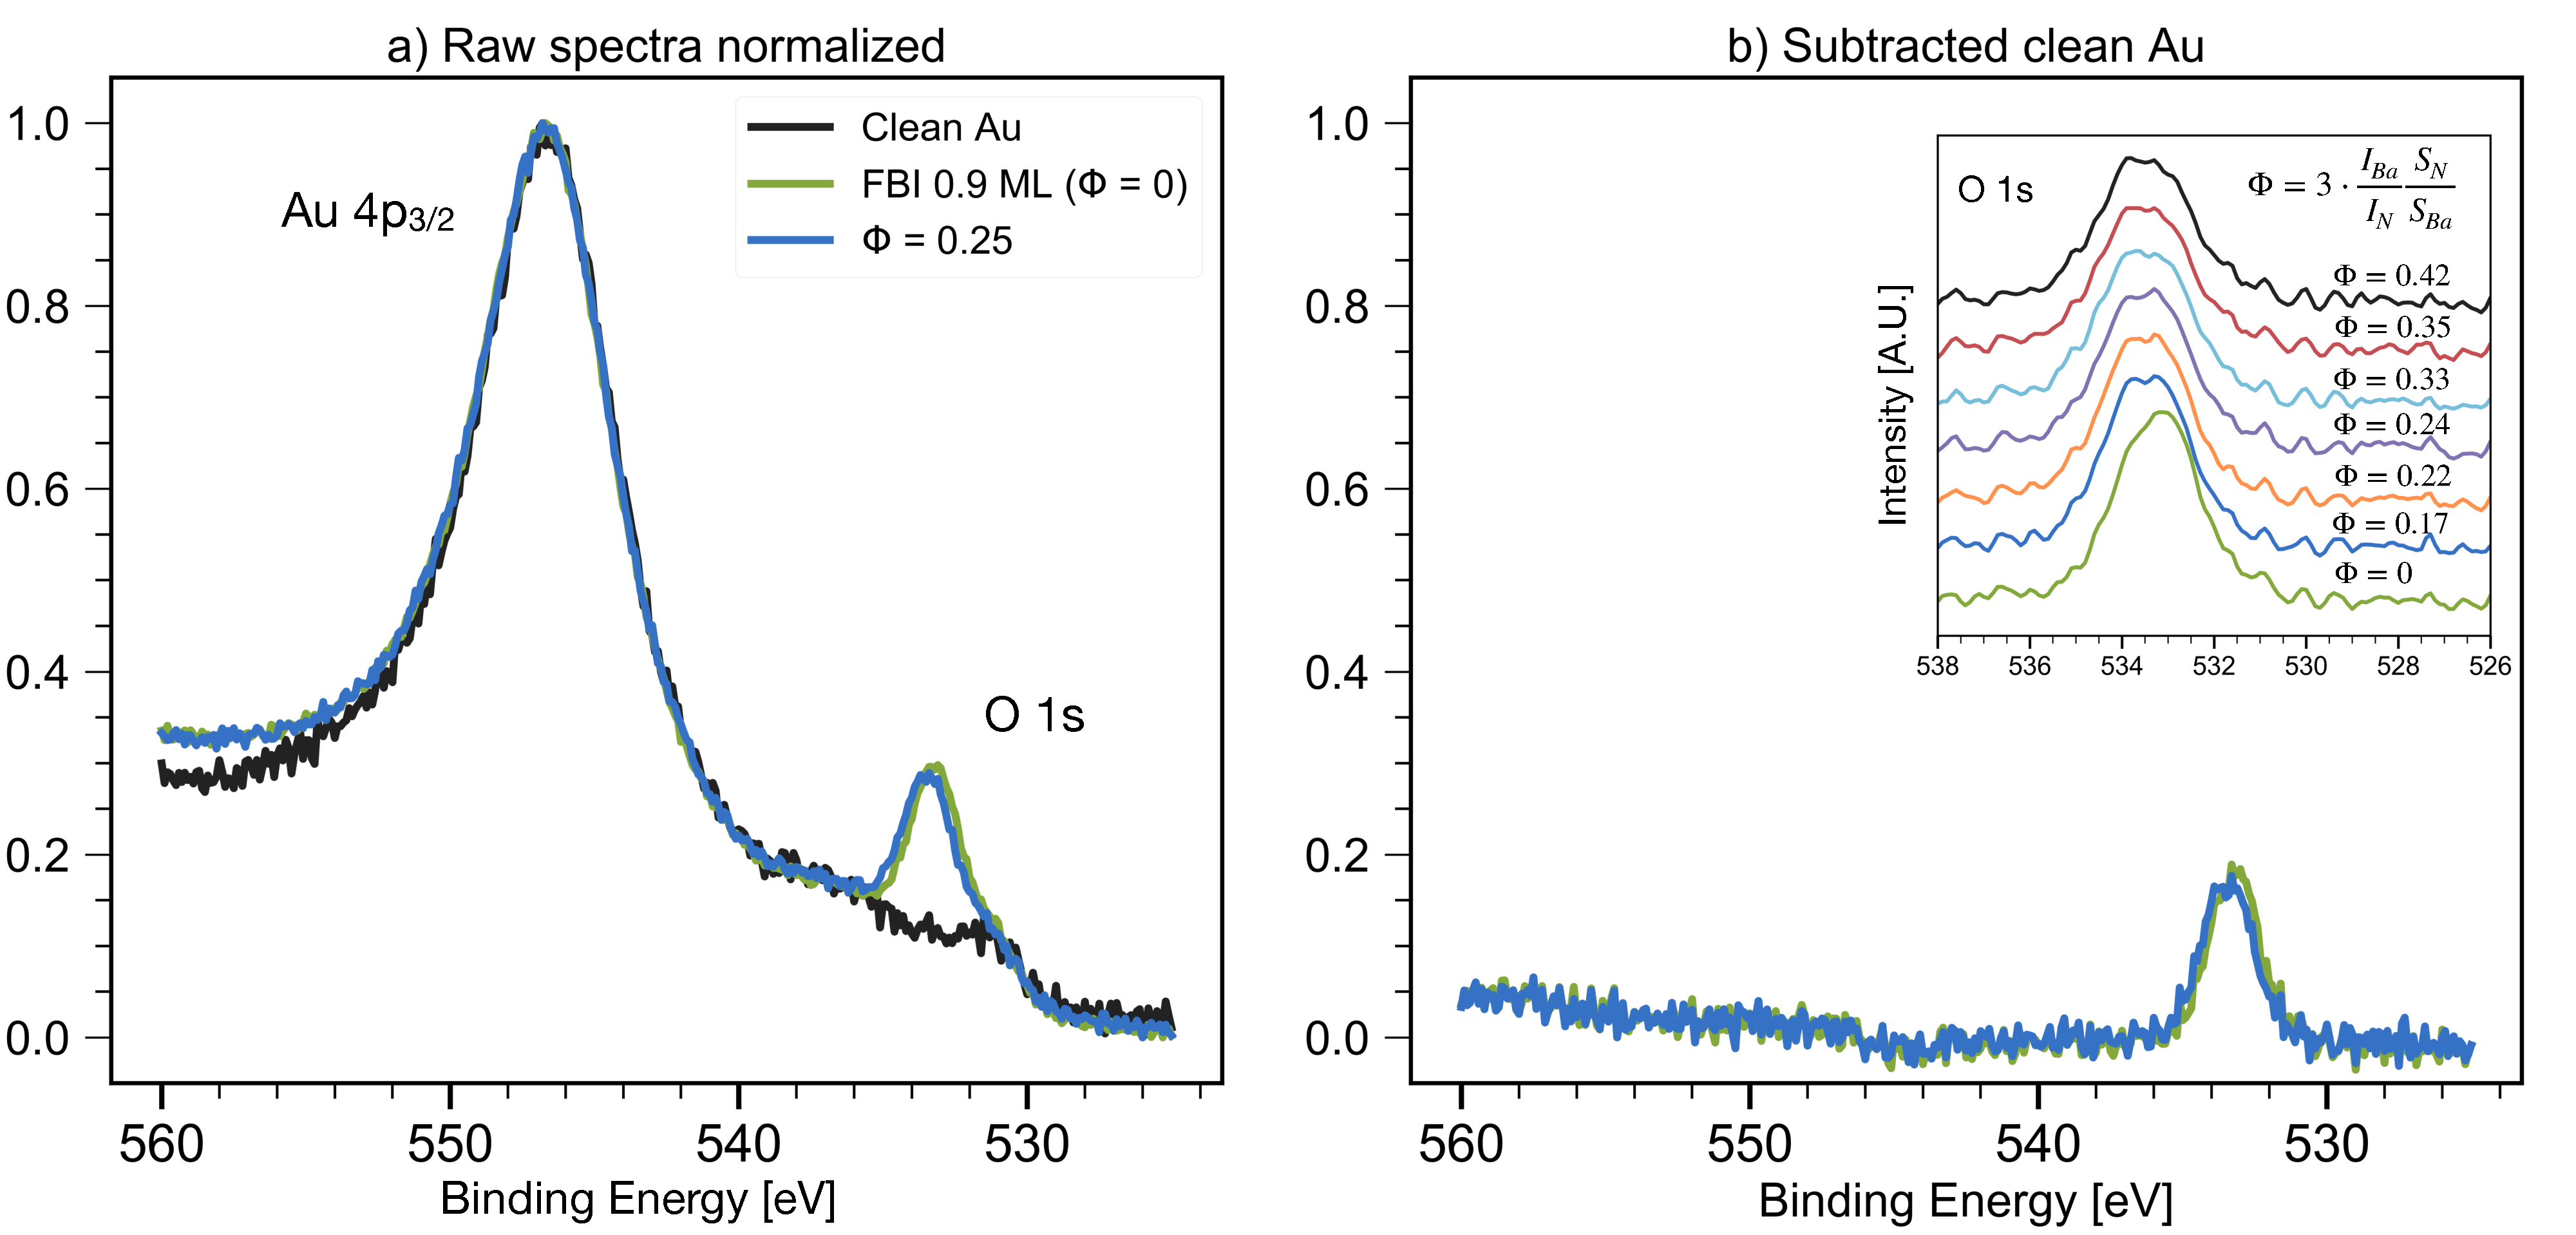
\includegraphics[width=0.9\textwidth]{figures/si_au_subtraction.png}
	\caption{\label{Au_subtraction} 
    XPS data treatment for O 1s core level in Au(111). The Au 4p core level contributes to the O 1s background. The intensity of the clean sample (red line) was subtracted from that corresponding to the deposition of FBI molecule (green line). To account for the attenuation of the Au 4p peak after evaporating the molecule, the maximum intensity of both curves was normalized to unity. The same treatment was applied to all lines in figure \ref{XPS_FBI_Au(111)} d). Those curves are shown here as inset with no offset.}
\end{figure*}  

\subsection{Calculation of the Ba:Cl stoichiometry after sublimation}

\begin{figure*}[ht!]
	\includegraphics[width=0.9\textwidth]{figures/si_bacl_au_cu.png}
	\caption{\label{Chlorine_desorption} 
    Evaporation of \BappCl directly (with no FBI molecule layer in between) on Cu(111) (black line) and Au(111) (red line). The stoichiometry ratio Cl/Ba, taking into account the atomic sensitivity factors (0.89 and 7.49 for Cl 2p and Ba 3d, respectively) is 0.7 and 0.64, for deposition in Au and Cu, respectively. Compare this to the expected ratio of 2 for the stoichiometric \BappCl salt.}
\end{figure*}  

\end{document}
